
\subsection{Importance of interventional distribution}
\label{intervention}

While preserving the conditional distribution seems to be the right way to explain the global behavior of dependent features, there is another important aspect: the use of interventional instead of observational expectation. Just keeping the conditional distribution without using an unrealistic combination of data points is not enough to recover the right effects of dependent variables. The need for interventional expectation in model-agnostic explainable techniques instead of observational has been already formally discussed in \cite{Janzing2020FeatureProblem} as a recommendation to researchers who intend to extend the \gls{SHAP} technique. 

The concept of interventional expectation was first introduced in the causality literature \cite{Pearl1993BayesianIntervention} aiming to elucidate the effect of manipulating a specific feature within a hypothetical scenario. In this context, the manipulation entails substituting the value of$x_1$ for that feature, while holding the values of all other features constant. Specifically, given $X={x_1, x_2,...,x_n}$ a function $f(X)$ that predict $Y$, the interventional expectation regarding $x_1$ is defined by using the "do-operator" through \(E[Y | do(X_{1} = x_{1})]\). The "do-operator" defined by Pearl allows researchers to formalize and analyze the causal effect of setting a variable \(X\) to a particular value \(x\), effectively simulating an intervention in the system.  

In the traditional statistical literature, the use of \gls{ME} plots have long been proposed as one of the reliable way to interpret models in place of the coefficients \cite{long1997regression}. The \gls{ME} corresponds to the average differences in the outcome when the features partially change from one specified value to another. The \gls{ME} uses the observed conditional distribution and does not extrapolate the joint distribution present in the data. However, \gls{ME} is not able to differentiate the effects of correlated variables as the changes in the outputs are computed while changing all dependent variables in tandem using the observed distribution.

To illustrate how the use of observed distribution in a highly correlated scenario fails to recover the individual role of features, Figure \ref{fig:extrapolation_rf} shows the same issue as Figure \ref{fig:extrapolation_lr}, where the predictive function has unexpected results when predicting outside of the training data envelope. Now, the output $Y$ is defined by $f(x) = x_1 + x_2^3$ and the data was fitted by the non-linear random forest algorithm, which might be able to detect the new cubic effect of $x_2$. In this case, differently from \gls{ALE} plot that correctly traces a linear effect to $x_1$ and an exponential effect to $x_2$ , \gls{ME} recovered the same effects for both variables. 

The tension between the use of observational and interventional distribution has also been discussed around the implementation of \gls{SHAP}. Some authors argue that the use of observed expectation can attribute importance to irrelevant features \cite{Janzing2020FeatureProblem, Sundararajan2020TheExplanation} while using interventional can lead to extrapolation issues. In \cite{Chen2020TrueData}, the authors suggest that there is no correct choice for this value function. Instead, the crux of the interpretation hinges on whether the aim is fidelity to the model or alignment with the data.

Within this context, \gls{ALE} technique emerges as a suitable tool for global explanations of feature effects to real applications, where variables are not independent. \gls{ALE} has a good balance of the tradeoff of being true to the model and true to the data, as it uses the interventional conditional expectation. In other words, \gls{ALE} takes advantage of interventions to break variable dependencies while adhering to the data joint distribution when computing effects by parts of the data.

\begin{figure}[ht!]
\centering
  \fcolorbox{gray}{white}{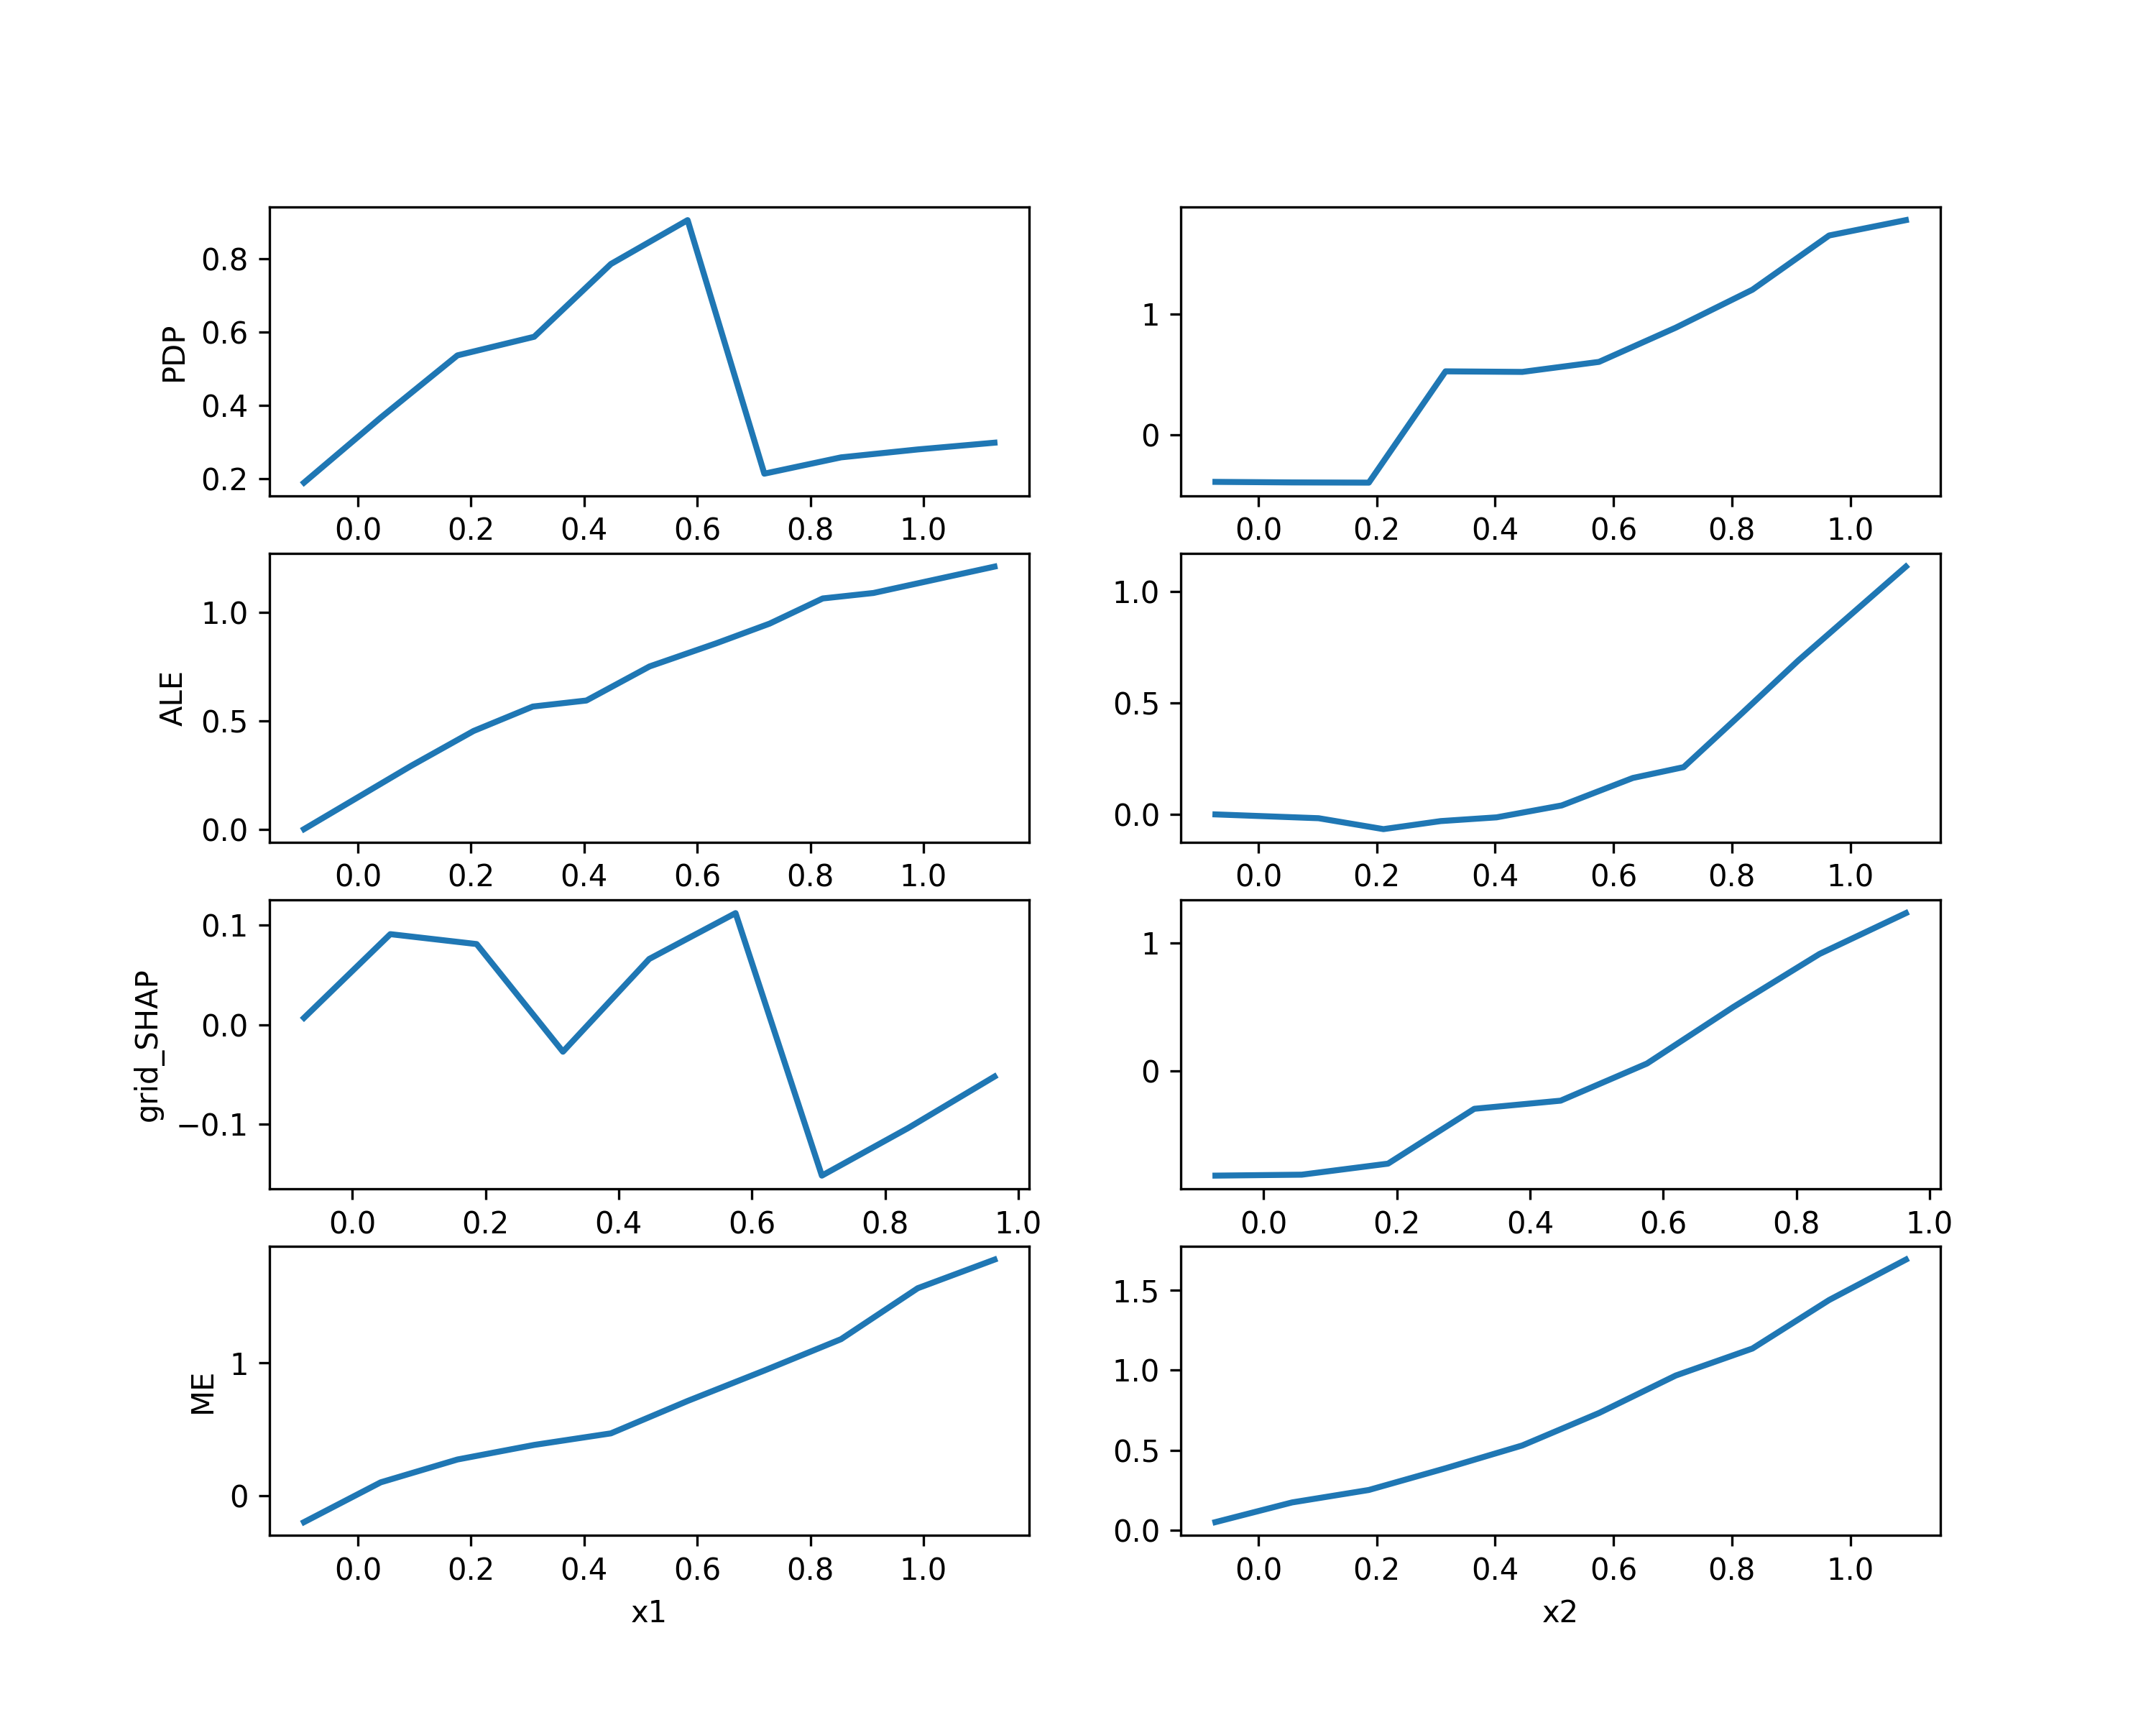
\includegraphics[width=0.98\textwidth]{images/extrapolation/extrapolation_rf.png}}
  \caption{Explanation of the customized random forest model for predicting a constant in a region beyond the training data bounds. The dataset was generated using the function $y = x_1 + x_2^3$}
    \label{fig:extrapolation_rf}
\end{figure}

